\chapter{Phenomenology of PDF determination}
\label{ch:3}

The aim of this chapter is to provide a brief review of the main methodological and numerical tools used in the determination of polarised parton distribution functions. In Sec.~\ref{sec:gen_fit_str} we delineate the general strategy for PDF determination, focusing on the phenomenological issues. We will pay special attention to the technical problematics that arise in the numerical implementation. Each issue will be then addressed in Sec.~\ref{sec:MAP}, in which we will present the methodologies adopted for the present analysis. The computational framework used to carry out the present work is provided by the MAP collaboration\footnote{
  \footnotesize{The GitHub page of the MAP Collaboration can be found at this link: \href{https://github.com/MapCollaboration}{https://github.com/MapCollaboration}.}
}. The code devoted to the determination of polarised PDFs, whose development has been the major work of this Thesis, goes by the name \texttt{Denali}.\par
The contents presented in this chapter will set the stage for Chap.~\ref*{ch:4}, in which the results will be discussed.

%___________________________________________________
\section{General approach to the global fitting}
\label{sec:gen_fit_str}

%%
\begin{figure}[t]
  \centering
  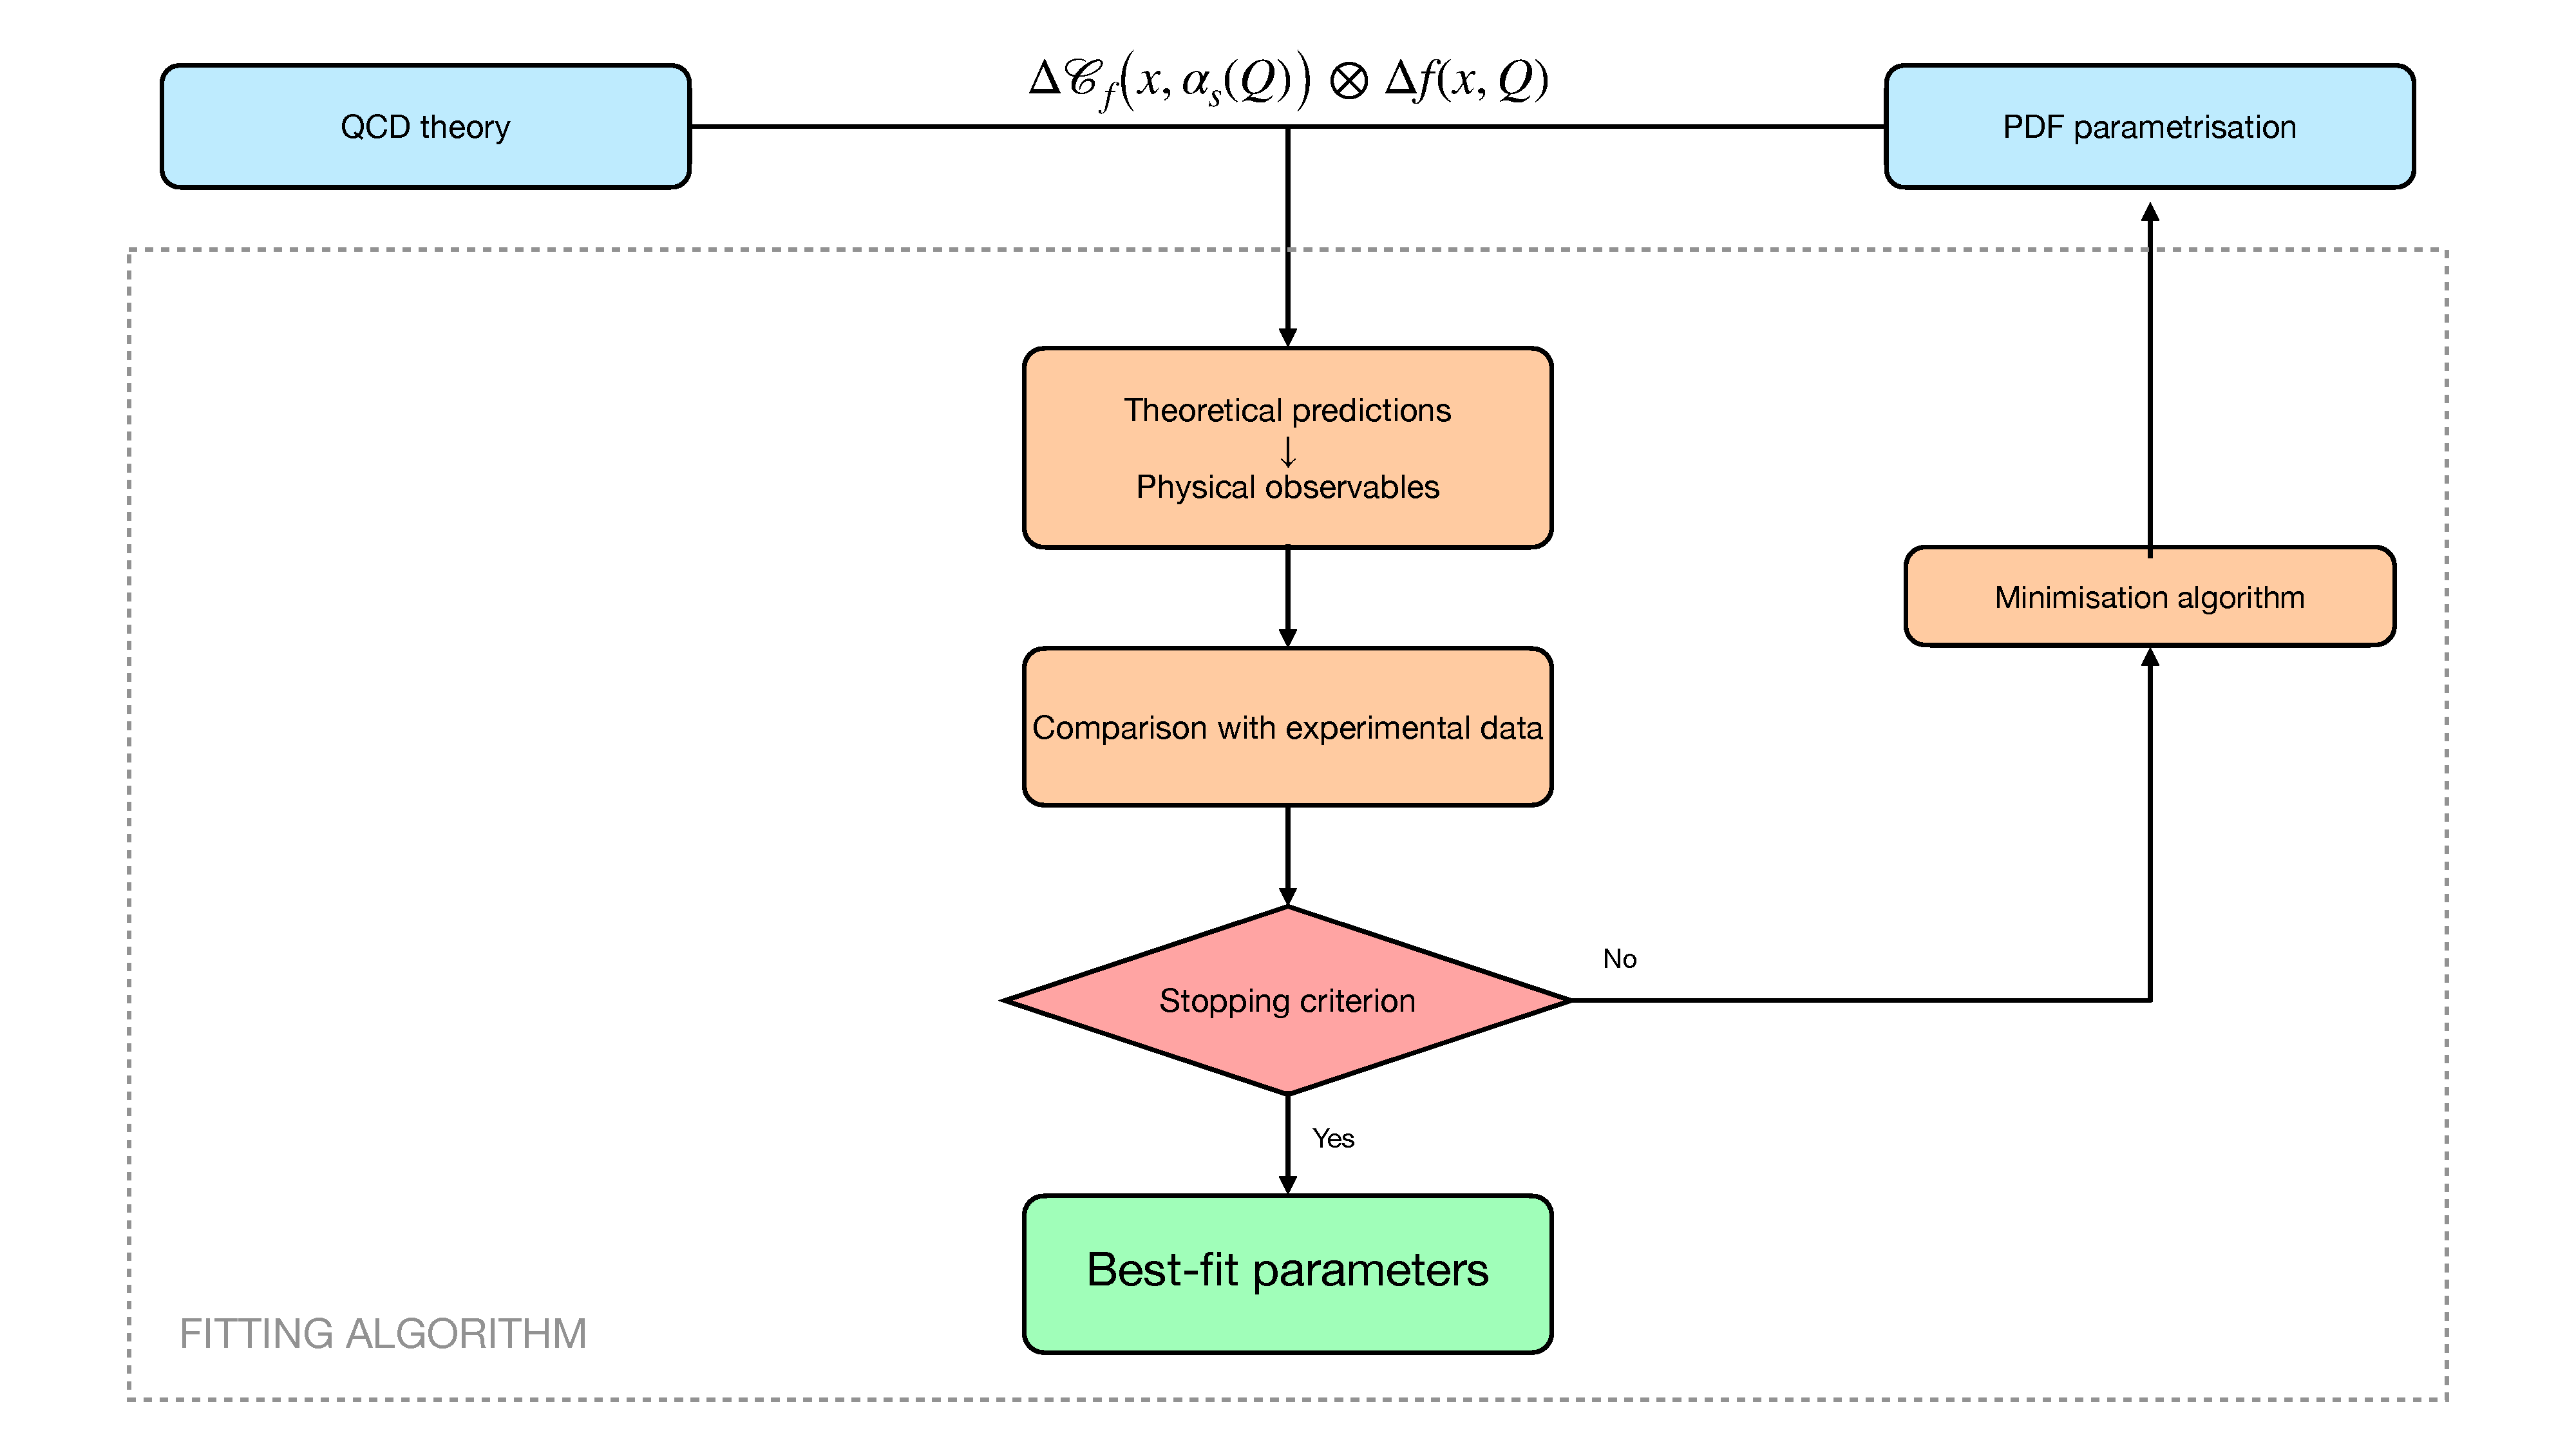
\includegraphics[width=1\textwidth]{fit_scheme.pdf} 
  \caption{Scheme of the general strategy for parton fitting.}
  \label{fig:fit_strategy}
\end{figure}
%%

Regardless the details of the adopted methodology, the general strategy for parton fitting can be summarised as in Fig.~\ref{fig:fit_strategy}. Starting from the top, the factorisation theorem allows for a net separation between the process-dependent contribution and the PDF. The former can be computed using the theoretical framework developed in Chap.~\ref{ch:2}, while the latter is parametrised by a certain function. Usually, the parametrisation of parton distributions is made at an initial energy scale $Q_0^2$, eventually evolved to the desired energy scale by means of the DGLAP equations, Eqs.~\eqref{eq:DGLAP_coupled}.\par
The set of measured observables $\left\{ \mathcal{O}^{\T{exp}}_i \right\}$ is compared with the corresponding set of theoretical predictions $\left\{ \mathcal{O}^{\T{th}}_i \right\}$. The agreement is quantified by a figure of merit (also known as \textit{error} or \textit{cost function}), usually chosen to be the $\chi^2$ function,
%%
\begin{equation}
  \chi^2 = \sum_{i,j}^{N_{dat}} \left( \mathcal{O}_{i}^{\T{(exp)}} - \mathcal{O}_{i}^{\T{(th)}} \right) \left[ \T{cov}_{ij} \right] \left( \mathcal{O}_{j}^{\T{(exp)}} - \mathcal{O}_{j}^{\T{(th)}}  \right) \,.
  \label{eq:chi2}
\end{equation}  
%%
where $\T{cov}_{ij}$ is the experimental covariance matrix. It is a block diagonal matrix due to the presence of correlated systematics, although the majority of polarised measurements are given with no correlated uncertainties. The reason for adopting the $\chi^2$ as error function relies on the assumption that data are independent and identically distributed, also known as \textit{i.i.d.} assumption. Then, Eq.~\eqref{eq:chi2} follows from the hypothesis that data are distributed according to a multivariate normal distribution, where the mean values are the experimental points and the covariance matrix is given by the experimental covariance matrix.\par
Finally, the best fit is obtained by minimising the cost function by means of an optimization procedure. The minimum is sought probing the parameter space until a stopping criterion decides whether the convergence is achieved or not. The best-fit parameters will eventually determine the shapes of the set of PDFs.\par
It should not surprise that the above picture, in spite of its apparent simplicity, hides several controversy complications. Moreover, despite each issue seems to  affect a precise part of the machinery, they are strongly related to each other, contributing all together to the efficiency of the algorithm. We summarise these several issues in the following list.\\[10pt]
%%
\begingroup
\textbf{Numerical implementation and theoretical assumptions.} The first problem that parton fitting faces is the implementation of the theoretical framework developed in Ch.~\ref{ch:2}. Indeed, a single observable requires the computation of several convolutions, which can be a highly time-consuming task if not addressed with attention. Moreover, parton distributions must be evolved to the required energy scale, introducing an additional degree of complexity to the computation. Finally, it must be noted that the coefficient functions to which the PDFs are convoluted with introduce non-regular distributions, such as Dirac delta functions or plus-prescriptions. We will provide a solution to these problems in Sec.~\ref{subsec:APFEL}.
\\[6pt]
Other theoretical subtleties may arise from the QCD analysis discussed in Sec.~\ref{sec:field_theoretic}. For instance, heavy quark mass effects have been completely neglected, as well as higher twist corrections. Such corrections are relatively small and their contributions can be mitigated by implementing \textit{ad hoc} kinematic cuts to the data set, as we shall see in Chap.~\ref{ch:4}
\\[6pt]
Moreover, several theoretical constraints can be adopted in order to improve the constraining power on the distribution and to speed up the algorithm. For instance, the sum rules, Eqs.~[\ref{eq:a3_PM}-\ref{eq:a8_PM}], provide an additional constraint to the first moments of the non-singlet quark combinations from the hyperon octet decay constants. However, these relations require the assumption of exact $SU(3)$ symmetry, which in principle can be violated, hence introducing a sort of bias in the determination. Other constraints will be discussed later, and we will check whether these assumptions introduce a sort of bias in our analysis.
\\[6pt]
Finally, it must be noted that the inclusion of processes involving identified hadrons in the final state introduces the dependence on the chosen set of FFs. For consistency, the perturbative order of the polarised PDF determination should match the perturbative order at which the FF determination has been carried out. The knowledge of these quantities and their uncertainties benefits the determination o polarised PDFs with a reliable uncertainty estimation.
\endgroup
\\[10pt]
\begingroup
\textbf{Limited experimental data.} Each experimental observable comes with its own definition in terms of precise combinations of parton distributions. This affects the final determination, since the fitting procedure will have more constraining power on those distributions (or combinations of them) that mainly contribute to the observable. In other words, each process allows for a different flavour separation. In this view, different processes bring complementary contributions to the analysis.
\\[6pt]
For instance, the major contribution to polarised data sets comes from polarised inclusive DIS data. As discussed in Chap.~\ref{ch:2}, the structure function related to this process only involves a particular combination of distributions, Eq.~\ref{eq:g1_NPM_ev}, mainly constraining the total quark distributions $\Delta u^{+}$, $\Delta d^{+}$ and $\Delta s^{+}$. However, it provides a mild contribution for the gluon distribution $\Delta g$, being it highly suppressed by the running coupling, Eq.~\eqref{eq:g1_QFT}.
\\[6pt]
Recently, SIDIS data with polarised beams and targets have been released, with different kind of species of identified hadrons (\textit{e.g.} $\pi^{\pm},K^{\pm}$). It is well known that the flavour of the originating parton, together with the charge of the hadron, strongly affect the FFs. As a consequence, it is possible to constraint alternative combinations of parton distributions by choosing the appropriate final hadron. It is then possible to achieve a full flavour decomposition for parton distributions. Still, the gluon contribution is note well constrained, given that it enters not at leading order.
\\[6pt]
Lastly, if compared with the unpolarised counterpart, polarised data are less precise and also less abundant, providing a rather limited kinematic coverage in the $(x,Q^2)$ plane. This has a strong impact on the final accuracy and precision of the determination.
\endgroup
\\[10pt]
\begingroup
\textbf{Functional parametrisation.} The choice of the parametrisation is the crux of the matter. Even though it can be made completely arbitrarily, given that PDFs represent our ignorance of the non-perturbative nucleon structure, the parametrisation has important impacts on the final results. The functional form can be chosen to naturally implement some known behaviour, such as the behaviour at small-$x$ as suggested by the Regge theory
or the exact cancellation of the distributions at $x=1$; or can also contain some theoretical constraints. However, it may be source of \textit{bias}, since it forces parton distributions to have a specific functional form. Moreover, also the number of free parameters that enter the functional form affects the analysis. A wider parameter space reflects in a more flexibility of the parametrisation, yet a trade-off must be taken into account: if the number is too high, the algorithm results to be too flexible, and will fit unwanted information of the data sets, such as the noise. On the other hand, a small parameter space reduces the flexibility, hence introducing a strong bias on the functional form of the determination.
\endgroup
\\[10pt]
\begingroup
\textbf{Error estimate.} Beside the functional parametrisation, another relevant issue is the PDF error determination. This can be achieved with the Hessian formalism \cite{Pumplin:2001ct}, or with the Lagrange multiplier method \cite{Stump:2001gu}. The former relies on the expansion about the minimum of the cost function, and requires the computation of the Hessian matrix, \textit{i.e.} the computation of the second derivative of the error function. On the other hand, the latter estimates the uncertainty by minimizing the error function with different values of a penality term. Both approaches involve massive computational tasks, either because of the difficulties encountered in computing the Hessian matrix, or because of the introduction of the penality term which strongly slows the speed of the fit. In addition, the Hessian method relies on the assumption that a first order, linear approximation is adequate, and error estimates based on this method are not necessarily always accurate.
\\[6pt]
A different approach is provided by the Monte Carlo sampling method, which is the one adopted for this analysis and will be discussed in Sec.~\ref{sec:MCS}. A comparison between these methods, with general details on each of them, can be found in Ref.~\cite{Forte:2010dt}.
\endgroup
\\[10pt]

\section{The MAP methodology}
\label{sec:MAP}
Having outlined the main issues involved, we are now ready to expose the methodology adopted to determine polarised PDF. The determination is based on a Monte Carlo approach and the functional parametrisation is given by a feed-forward neural network (NN). The Monte Carlo sampling addresses the problem of the uncertainty estimation for all the observables related to polarised PDFs, while the NN provides an unbiased and flexible parametrisation of the distributions. The computation of the theoretical observables is handled by the \texttt{APFEL++} library, which tabulates the integrals that enter the analysis to create the so-called FK tables. Finally, stochastic gradient descent (SGD) and cross-validation are used to train the network, avoiding the problem of \textit{overfitting}. A description of these tools is presented in the sections below.

\subsection{Numerical implementation: the \texttt{APFEL++} library}
\label{subsec:APFEL}
One of the issues that concerns a global analysis is the numerical implementation of theoretical framework discussed in Chap.~\ref*{ch:2}. In \texttt{Denali}, convolutions and evolutions are handled by the \texttt{APFEL++} \cite{Bertone:2016lga,Bertone:2017gds}, whose methodology we shall briefly discuss here.\par
In the context of collinear factorisation, the most relevant quantity that we have to compute is a Mellin convolution between an operator $\mathcal{O}$ and a distribution $d$, which we report here for convenience:
%%
\begin{equation}
  \mathcal{M}(x) = \int_{0}^{1} dy \int_{0}^{1} dz \; \mathcal{O}(y) d(z) \delta(x-yz) = \int_{x}^{1} \frac{dy}{y} \mathcal{O}(y) \left( \frac{x}{y} \right)\,.
  \label{eq:def_conv2}
\end{equation}
%%
We will use $\mathcal{M}(x) \equiv \mathcal{O}(x) \otimes d(x)$ as shorthand notation for the convolution. The operator $\mathcal{O}$ contains the process-dependent perturbative contributions. Although its expression may become complicated at higher perturbative orders, it always shows the same mathematical structure: a "regular" term, whose integration into Eq.~\eqref{eq:def_conv2} does not present any difficulty, "local" terms proportional to $\delta(1-x)$, and "singular" terms, in which the singularity in $x=1$ is subtracted by means of the so-called plus-prescription. Such a complex structure makes the computation of Eq.~\eqref{eq:def_conv2} rather expensive. On the other hand, the distribution $d$, which is the subject of interest in the present analysis, does not present any complication and can be easily accessed through the LHAPDF interface \cite{Buckley:2014ana}.\par
In order to make the computation of the integral \eqref{eq:def_conv2} fast, the standard strategy is to use interpolation techniques and precompute the expensive part of the integral. First, the integration variable $z$ is discretised on a grid $g=\left\{ z_0,\dots, z_N\right\}$. Then, the distribution $d$ is interpolated over the grid $g$ by means of a set of interpolating functions:
%%
\begin{equation}
  d(z) = \sum_{\beta \in g} w_{\beta}(z) d_{\beta} \,,
  \label{eq:inter}
\end{equation}
%%
where $d_{\beta} \equiv d(z_{\beta})$ is the distribution $d$ evaluated on the interpolating point $z_{\beta}$ of the grid, whereas $w_{\beta}$ is the interpolating function associated to the $\beta$-th node. Usually, Lagrange polynomials are chosen as interpolating functions. After inserting Eq.~\eqref{eq:inter} into Eq.~\eqref{eq:def_conv2}, and assuming the value of $x$ to be equal to the $\alpha$-th node of the grid, the quantity $\mathcal{M}$ evaluated at $x_{\alpha}$ may be computed as a simple matrix product
%%
\begin{equation}
  M_{\alpha} \equiv M(x_{\alpha}) = \mathcal{O}_{\alpha \beta} d_{\beta} \,,
  \label{eq:vec_obs}
\end{equation}
%%
where the matrix $\mathcal{O}_{\alpha \beta}$ has been defined as
%%
\begin{equation}
  \mathcal{O}_{\alpha \beta} \equiv \int_{x_{\alpha}}^{1} \frac{dy}{y} \mathcal{O}(y) \, w_{\beta} \left( \frac{x_{\alpha}}{y}  \right) \,.
  \label{eq:matr_O}
\end{equation}
%%
In both Eqs.~[\ref{eq:vec_obs}-\ref{eq:matr_O}] a sum over repeated Greek indices is understood. Then, we can access an arbitrary value for $\mathcal{M}$ through the same interpolation technique:
%%
\begin{equation}
  M(x) = \sum_{\alpha \in g} w_{\alpha}(x) M_{\alpha} \,.
\end{equation}
%%
Hence, the integral Eq.~\eqref{eq:matr_O} can be tabulated once and for all, the computaion of the observable $\mathcal{M}$ just amounts of a simple multiplication between a matrix and a vector. The operation thus becomes very fast and can be easily extended to any other distribution $d$.\par 
We observe that the computation of an observable and the evolution share the same mathematical structure of Eq.~\eqref{eq:def_conv2}. Hence, both tasks can be recast into a unique set of tabulated values, providing the so-called Fast-Kernel (FK) tables.

\subsection*{Solution to DGLAP equations}
In Sec.~\ref{sec:field_theoretic} we have introduced the DGLAP equations, a set of $(2 n_f + 1)$ integro-differential equations that describe the evolutions of PDFs (and FFs) with the scale $Q^2$. The kernel of this set of equations can be calculated in perturbative QCD, and at any order the mathematical structure is unchanged. Schematically, the equations can be written as 
%%
\begin{equation}
  \pdv{\Delta f_i(x, Q^2)}{\ln Q^2} = \int_x^1 \frac{dy}{y} P_{ij} \qty(\frac{x}{y}, Q^2) \; \Delta f_j(y,Q^2) \, ,
  \label{eq:DGLAPs}
\end{equation} 
%%
where the factor containing the coupling constant has been neglected and the factors in the RHS of Eq.~\eqref{eq:DGLAP_coupled} is contracted into a single term $P_{ij}$. In the following, the latin indexes run over quark and antiquark flavours together with the gluon ($i=u,d,\dots \bar{u},\bar{d}, \dots g$), whereas the greek indexes run over the nodes of the grid $g$.\par
We can apply the same interpolation technique and interpolate the distribution $\Delta q_{i}(x,Q^2)$ as we did in Eq.~\eqref{eq:inter}. In doing so, Eq.~\eqref{eq:DGLAPs} acquires a simple form
%%
\begin{equation}
  \pdv{\Delta f_i(x_{\alpha},Q^2)}{Q^2} = \sum_{\beta} \Pi_{ij,\alpha \beta} (Q^2) \; \Delta f_j(x_{\beta}, Q^2) \,,
  \label{eq:DGLAP_recast}
\end{equation}
%%
where the matrix $\Pi_{ij,\alpha \beta}$ is defined as in Eq.~\eqref{eq:matr_O} and reads
%%
\begin{equation}
  \Pi_{ij,\alpha \beta} (Q^2) = \int_{x_{\alpha}}^1 \frac{dy}{y} P_{ij} \qty(\frac{x_{\alpha}}{y}, Q^2) \; w_{\beta}^{(k)} (y)\,.
\end{equation}
%%
The functions $w_{\beta}^{(k)}$ are Lagrange polynomial of degree $k$ used as interpolating function. We can assume that $\Delta f_i(x_{\beta},Q^2) \equiv \Delta f_{i,\beta}(Q^2)$ evolves between the energies $Q^2$ and $Q^2_0$ according to
%%
\begin{equation}
  \Delta f_{i,\beta} (Q^2) = \sum_{k} \sum_{\gamma} \Gamma_{ik,\beta \gamma} (Q^2,Q^2_0) \, \Delta f_{k,\gamma} (Q^2_0) \,,
  \label{eq:disc_evol}
\end{equation}
%%
provided that the boundary condition $\Gamma_{ik,\beta \gamma} (Q^2,Q^2_0) = \delta_{ik} \delta_{\beta \gamma}$ is satisfied. The evolution operator in Eq.~\eqref{eq:disc_evol} satisfies the following differential equation
%%
\begin{equation}
  \frac{\partial \Gamma_{ij,\alpha \beta} }{\partial \ln Q^2} (Q^2,Q^2_0) = \sum_{k} \sum_{\gamma} \Pi_{ik,\alpha \gamma}(Q^2) \, \Gamma_{kj,\gamma \beta}(Q^2,Q^2_0)  \,,
  \label{eq:sys_DGLAP_kernel}
\end{equation}
%%
which is a first order linear differential equation. It can be solved with standard numerical algorithms, such as the Runge-Kutta methods.\par

\subsection*{Fast-Kernel tables}
We have all the ingredients to present the numerical implementation of the calculations of the structure functions. In the framework of DIS, the polarised structure function $g_1$ can be decomposed as 
%%
\begin{equation}
  \begin{split}
    g_1(x,Q^2) & = \sum_{i=q,\bar{q},g} \Delta \mathcal{C}_{i}(x,Q^2) \otimes \Delta f_i (x,Q^2) \\
    & = \sum_{i=q,\bar{q},g} \Delta \mathcal{C}_{i}(x,Q^2) \otimes \Gamma_{ij} (Q^2,Q^2_0) \otimes \Delta f_i (x,Q^2_0) \,,
  \end{split}
\end{equation}
%%
where $\Delta \mathcal{C}_{i}(x,Q^2)$ are the process-dependent coefficient functions that we discussed in Sec.\ref{sec:field_theoretic}. $\Gamma_{ij} (Q^2,Q^2_0)$ is the evolution operator that we introduced earlier and that evolves the distribution from the initial parametrisation scale $Q^2_0$ to the hard-scattering scale $Q^2$. Finally, $\Delta f_i$ is the polarised PDF of flavour $i$ evaluated at the initial scale $Q^2_0$ and $\otimes$ denotes the usual Mellin convolution, Eq.~\eqref{eq:def_conv2}. Since the direct calculation is numerical expensive, we can exploit the methodologies previously discussed. Indeed, 
%%
\begin{equation}
  \begin{split}
    g_1 (x_{\alpha},Q^2) & = \sum_{i} \mathcal{O}_{i,\alpha \beta}(Q^2) \Delta f_{i,\beta}(Q^2) \\
    & = \sum_{i,k} \sum_{\beta, \gamma} \mathcal{O}_{i,\alpha \beta}(Q^2) \Gamma_{ik,\beta \gamma} (Q^2,Q^2_0) \Delta f_{k,\gamma}(Q^2_0) \\
    & = \sum_{k} \sum_{\gamma} \left( FK \right)_{k, \alpha \gamma} (Q^2,Q^2_0) \Delta f_{k, \gamma}(Q^2) \,,
    \label{eq:g1_FK}
  \end{split}
\end{equation}
%%
where the information about the partonic cross-sections and the DGLAP evolution are encoded into the FK tables, defined as
%%
\begin{equation}
  FK_{k, \alpha \gamma}  (Q^2, Q^2_0) \equiv \sum_i \sum_{\beta} \mathcal{O}_{i,\alpha \beta}(Q^2) \Gamma_{ik,\beta \gamma} (Q^2, Q^2_0)\,.
\end{equation}
%%
As a result, the series of convolutions are expressed in terms of simple matrix multiplications that can be easily handled inside a code. Moreover, the tabulation of the FK tables can be done once and for all at the beginning of the fit, improving the speed and the memory efficiency of the algorithm. The result is the elegant factorisation of the polarised PDFs at the input scale $Q^2_0$, Eq.~\eqref{eq:g1_FK}, which is the quantity that we parametrise.\par
In case of double convolutions, as for the SIDIS observables, this procedure still holds. It turns out that the coefficient functions for SIDIS have a net separation of the kinematic variables $x$ and $z$, concerning the PDFs and the FFs, respectively. Hence, the double convolution is simply transformed into a product of two convolutions, each of them bearing separately the dependence either on $x$ on in $z$. 


%___________________________________________
\subsection{Neural Network parametrisation}
\label{sec:NN}

In \texttt{Denali}, polarised PDFs are parametrised in terms of a neural network. In the context of PDF determination, neural networks have been used for the first time by the NNPDF collaboration \cite{Forte:2002fg}. For the current analysis, we will deal with feed-forward neural network, although other structure can be obtained (see \textit{e.g.} \cite{Bishop}). The part of the code concerning the parametrisation with neural networks, and that also provides an efficient way to compute the analytic derivatives, is handled by \texttt{NNAD} \cite*{AbdulKhalek:2020uza}.\par
Neural networks are neural inspired nonlinear model for supervised learning. Basically speaking, neural network models can be regarded as a series of nonlinear transformations. The building blocks of a network are the \textit{neurons} (or $\textit{nodes}$), organised in \textit{layers}, with the output of one layer serving as the input for the next. The first layer of the network is the \textit{input} layer, whereas final one corresponds to the \textit{output} layer. All the layers in the midst are called \textit{hidden units} (or \textit{hidden layers}).\par
Starting from input layer, we can construct $N_1$ linear combinations of the input variables $x_1, \dots, x_N$ and obtain:
%%
\begin{equation}
  a_j = \sum_{i=1}^{N} w_{ij}^{(1)} x_i + \theta^{(1)}\,,
  \label{eq:activation}
\end{equation}
%%
where $j=1,\dots,N_1$ and the subscript $(1)$ indicates that the corresponding parameters are related to the first layer (the one immediately after the input layer) of the NN. The parameters $w^{(1)}_{ji}$ are usually known as \textit{weights} and the parameters $\theta^{(1)}$ as \textit{biases}. Together with the input variables, they participate in the construction of the quantity $a_j$, also known as $activation$. The latter serves as argument of a differentiable, nonlinear \textit{activation function} $h$ to give
%%
\begin{equation}
  z_{j} = h(a_j)\,,
\end{equation}
%%
hence providing a functional (nonlinear) transformation of the activation. The outputs of these transformations serve as input for the nodes that compose next layer.\par The procedure that we have just discussed can be iterated, provided that a new set of weights and biases in introduced. Given a NN with $L$ layers and $N_{\ell}$ nodes in the $\ell$-th layer, the output of the $i$-th neuron in the $\ell$-th hidden layer can be written as
%%
\begin{equation}
  z_{i}^{(l)} = h \left( \sum_{j=1}^{N_{l-1}} w_{ij}^{(l)} z_{j}^{(l-1)} + w_{i0}^{(l)} \right) \,,
  \label{eq:activity}
\end{equation}
%%
In the terminology adopted, the input layer is denoted by $l=1$, the output layer with $l=L$, and the hidden layers with $l=2,\dots,L-1$.\par
%Both weights and parameters can be seen as synapsis, that is connections between two pairs of neurons in subsequent layers.\par
In order to properly approximate a continuous function, the activation functions must be nonlinear. Indeed, if all the hidden units in the network were taken to be linear, then it would be possible to find a single linear transformation equivalent to the network. This is a direct consequence of the fact that the composition of successive linear transformations is itself a linear transformation. The simplest example of activation function is the step function $\Theta(x)$, which acts as a binary activator. With this choice, the neural network can be seen as made of multiple layers of \textit{perceptrons}, discriminative functions in linear models for classification. For this reason, the name \textit{multilayer perceptron} is used to indicate this type of configuration. However, one is led to use continuous nonlinear functions instead of step-function nonlinearities. In doing so, the neural network becomes differentiable with respect to the parameters. This property is fundamental in network training, and it is exploited by \texttt{NNAD} for computing the gradient of the network over the parameter space. The most popular activation function is the sigmoid
%%
\begin{equation}
  h(a) = \frac{1}{1 - e^{-a}}\,,
  \label{eq:sigmoid}
\end{equation}
%%
which presents two distinct regimes — linear and nonlinear. The linear response is obtained when the argument is approximatively near the origin, $a \approx 0$, whereas it saturates for large positive and negative values. If the parameters are such that the sigmoid works on the crossover between linear and saturation regimes, the nonlinearity of the NN is restored.\par
Globally, a neural network can be seen as a function of the set of weights $\{ w^{(l)}_{ij} \}$ and biases $\{ \theta_{i}^{(l)} \}$, together with the inputs $\left\{  x_i\right\}$
%%
\begin{equation}
  \vb*{z}^{(L)} \equiv f \left( \vb*{w}, \vb*{x}; \, h \right) \,.
  \label{eq:NN_func}
\end{equation}
%%
The process of evaluating Eq.~\eqref{eq:NN_func} is a forward propagation, since the information of the input layer is propagated through the network with continuous transformations. For that reason, such an architecture is known as \textit{feed-forward neural network}. It must be observed that we consider only neural network in which the previous layer is connected only with the consecutive layer. Other feed-forward topology, however, are possible.\par
The choice of the activation function in the output layer is determined by the nature of the problem that we are addressing. Among many possible options, the most popular are linear functions, sigmoid, or the identity. However, in the next chapter we will see that this arbitrariness allows to choose the output function in order to implement physical constraints analytically, improving the efficiency of the algorithm.\par
Given the high number of parameters that enter the neural network, the functional form is redundant enough not to introduce a theoretical bias which would artificially reduce parton uncertainty in regions where data do not constrain enough PDFs.


%______________________________________________
\subsection{Network training and optimisation}
\label{sec:NNtr}
After defining the general structure of the network parametrisation, we now address the delicate issue of finding the set of parameters that best approximates the data (and also gives good predictions). In the context of neural network, the optimisation of the parameter space is also known as \textit{network training}. The first step of the network training is the minimisation of the error function. Since it is a smooth continuous function of the parameters, its smallest value occurs at point in parameter space such that the gradient of the error function vanishes. However, given the high nonlinearity of the error function w.r.t. the parameters, there could be different local minima. Since it is clearly impossible to find an analytical solution to the equation $\nabla \chi^2 = 0$, we must resort to iterative numerical procedures that probe the space of parameters. The basic idea is that a small step in weight space reflects in the change in the error function. Thus, in order to find the minimum of the error function, we can start from a random initialised set of parameters and then move through the weight space in a succession of steps. The standard choice is to use the so-called gradient descent (GD) method, in which the minimum is sought by moving along the direction of the negative gradient of the cost-function
%%
\begin{equation}
  \vb*{w}^{\tau + 1} = \vb*{w}^{\tau} - \eta \nabla \chi^2 (\vb*{w}^{(\tau)}) \,,
  \label{eq:GD}
\end{equation}
%%
where $\tau$ label the iteration step and $\eta$ is the \textit{learning rate}. However, for our analysis we adopt the stochastic gradient descent (SGD). Stochasticity is incorporated by computing the gradient on a subset of the data called \textit{minibatch}. The impact of this variation of GD method is twofold: first, it introduces stochasticity and decreases the chance that the fitting algorithm gets stuck in isolated local minima. Second, it significantly speeds up the calculation as one does not have to use all the data points to approximate the gradient.\par
The reason that led us to use gradient information in the minimisation procedure is that the gradient of the error function can be computed efficiently by means of the \textit{backpropagation} procedure. It relies on the ordinary chain rule for partial differentiation. Indeed, the cost function depends directly on the activities of the output layer $z_j^{(L)}$, but also indirectly on all the activities of neurons in lower layers through iteration of Eq.~\eqref{eq:activity}. Hence, the gradient of the cost function w.r.t. the weights and biases of each layer can be obtained by applying consecutively the chain rule through the network, starting from the output layer. In other words, we are "backpropagating" the error starting with the top layer down to the input layer and uses these intermediate errors to calculate the desired gradients \cite{HBLV}. Of course, this technique requires the knowledge of the derivative of the cost function with respect to the activities of the output layer, which is not always the case. However, it can be shown that using the $\chi^2$ as error function, a close and analytical expression for the gradient does exist \cite{AbdulKhalek:2020uza}. Such a computational efficiency is fundamental since the gradient must be computed at each step of the gradient descent.\par
Finally, we observe that the purpose of a neural network is not only approximation, but also prediction. That is to say, we want the predictions of the network to be comparable with a set of data the has not been use for the training. This is correlated to another subtle problem, known as \textit{overlearning}, due to the high redundancy and flexibility of the network. In presence of overlearning, it starts to fit statistical noise of the data, rather than the underlying physical law. This affects the prediction power, since the statistical noise is characteristic of each data set. The solution to this additional complication is achieved using a cross-validation method, which introduces a criterion that stops the fit before it starts over-learn. The technical details for this implementation will be discussed in Sec..


%___________________________________________
\subsection{Monte Carlo sampling}
\label{sec:MCS}
%%
\begin{figure}[t]
  \centering
  \begin{subfigure}[b]{0.45\textwidth}
      \centering
      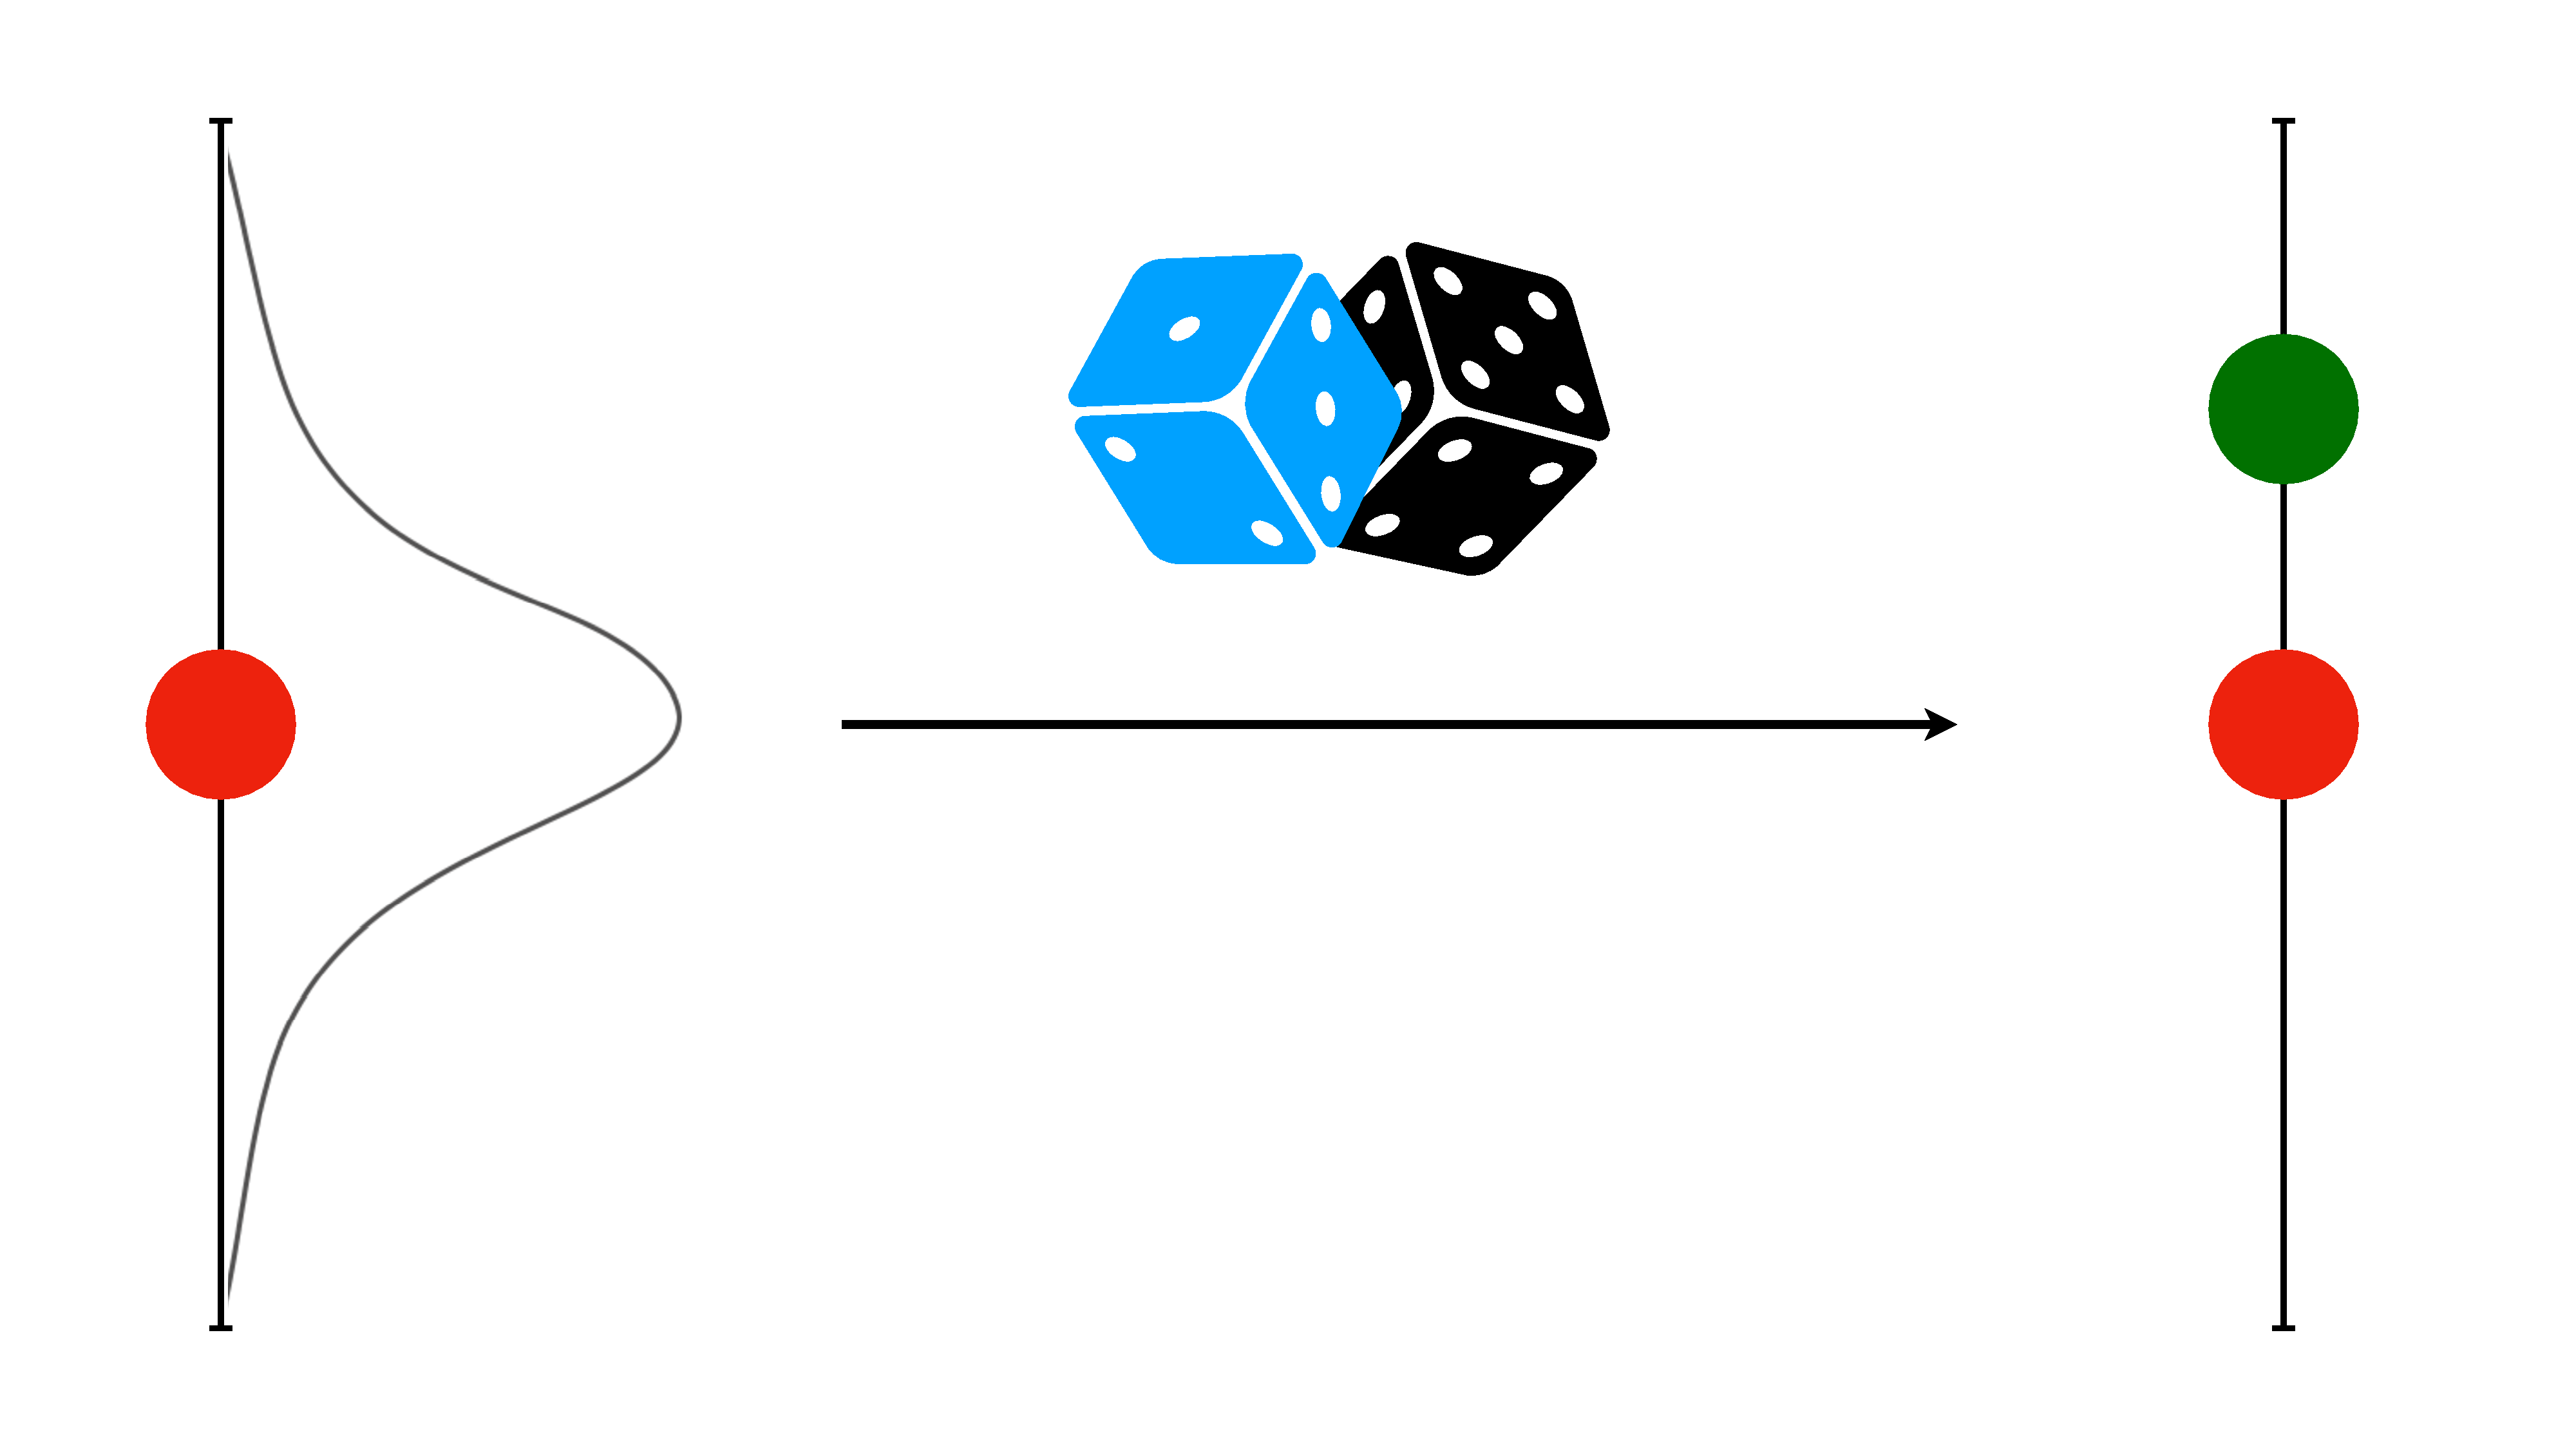
\includegraphics[width=\textwidth]{MC_fluc.pdf}
      \caption{The fluctuation process. The red dot is the central value; the green dot is the artifical value.}
      \label{fig:MC_fluc}
  \end{subfigure}
  \hfill
  \begin{subfigure}[b]{0.45\textwidth}
      \centering
      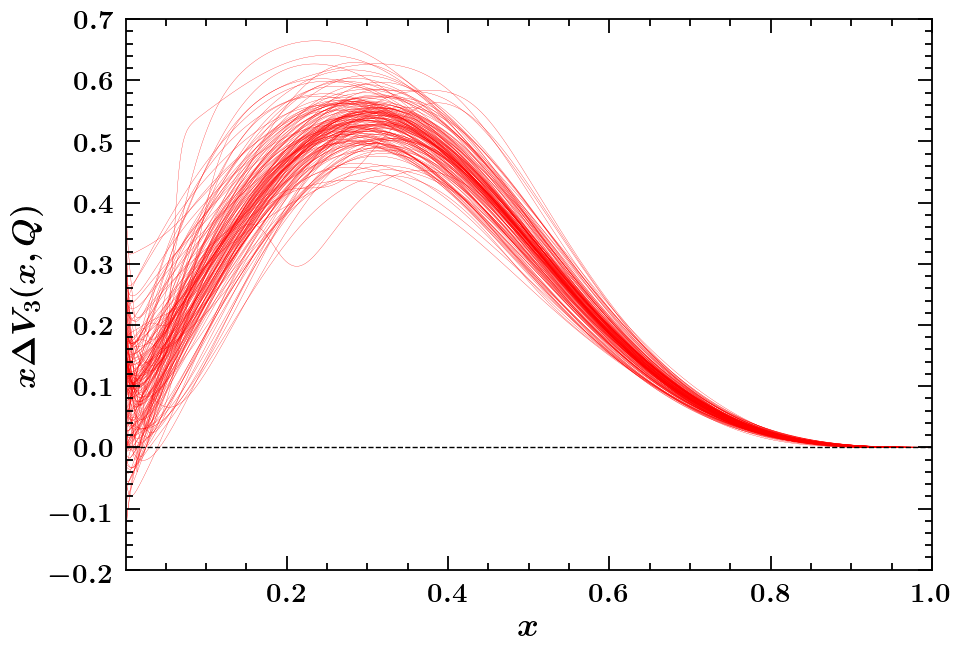
\includegraphics[width=\textwidth]{replica.png}
      \caption{Ensemble of polarised PDFs.}
      \label{fig:PDF_ensemble}
  \end{subfigure}
     \caption{Representation of the Monte Carlo Sampling}
     \label{fig:MC_2_Gr}
\end{figure}
%%
The average of an observable the depends on polarised PDFs $\mathcal{O}(\Delta f_i)$ is given by integrating the observable itself in the functional space $\mathcal{V}\left( \left\{ \Delta f_i \right\}\right)$ spanned by the parton distributions, weighted by the probability measure $\mathcal{P}\left(\{\Delta f\}\right)$ to observe a PDF at some reference scale, that is \cite*{Nocera:2014vla}
%%
\begin{equation}
  \left< \mathcal{O}(\Delta f) \right> = \int_{V} \mathcal{D} \Delta f \; \mathcal{P}{\Delta f} \; O \left[ \Delta f \right] \,.
\end{equation}
%%
We have no hope of finding an analytical expression for the probability measure $\mathcal{P}{\Delta f}$. However, we can sample the distribution by a Monte Carlo method.\par
First, we generate an ensemble of replicas of the original data set, following the statistical distribution of the experimental data. Each artificial ensemble contains as many data points as are originally available in the data set. The process of creating the artificial data points from the distribution of the experimental data is called fluctuation. We will refer to the original set as the the unfluctuted data set. The statistical distribution of the experimental data contain all the experimental information, that is statistical and systematic uncertainties. In practice, most data are given with mulivariate normal distributions, in which the uncertainties are contained in the covariance matrix and the mean value corresponds to the experimental central value. A sketch of the fluctuation procedure is shown in Fig.~\ref{fig:MC_fluc}. The number of replica is chosen to faithfully reproduce the statistics of the original set, by means of statistical estimators that will be discussed in Sec..\par
Then, for each artificial ensemble, parton distributions are fitted to the fluctuated data. Thus, at the end of the fit, one obtains a collection of PDFs with as many members as the number of replicas $N_{rep}$ generated from the data, Fig.~\ref{fig:PDF_ensemble}. Of course, each PDF replica will fluctuate accordingly to the fluctuated data set used for the fit. However, this collection of PDFs replica serves as a statistical ensemble, from which one can compute the central value and the one-sigma uncertainty. The smoothness of these two estimators increases with the number of artificial sets generated for the global fit. The advantages of the Monte Carlo methodology go further. Indeed, the expectation value of any observable that depends on polarised PDFs can be easily computed by averaging over the PDF ensemble to obtain
%%
\begin{equation}
  \left< O\left[ \Delta f \right] \right> = \frac{1}{N_{\T{rep}}} \sum_{k=1}^{N_{\T{rep}}} O\left[\Delta f_k\right] \,,
\end{equation}
%%
where $O\left[\Delta f_k\right]$ is the value of the observable computed out of the k-th PDF replica. In the same fashion, one can compute uncertainties such as the standard deviation.\par
Finally, we observe that the optimisation procedure discussed in Sec.~\ref{sec:NNtr} must be performed for each replica. This expensive task, however, does not rely on any assumption, contrary to the Hessian method. Moreover, parallel processing is able to handle multiple fits simultaneously, reducing drastically the time required by a single global analysis.

